\documentclass[11pt,french]{report}
  \usepackage{babel}
  \usepackage{amsmath,amsfonts,amssymb}
  \usepackage[utf8]{inputenc}   % LaTeX
  \usepackage[T1]{fontenc}      % LaTeX
  \usepackage[autolanguage]{numprint}
  \usepackage{graphicx} %image
  	\graphicspath{{./fig/}} %fig path
  \setcounter{secnumdepth}{3} %profondeur de la numérotation du TOC
  \usepackage[colorlinks]{hyperref} %lien hypertex
  \usepackage{titlesec}	%package pour modifier les chapitres #2
  \usepackage[autolanguage]{numprint}
  \usepackage{tikz}
  \usepackage{tabularx}
  \usepackage{multirow}
  \setlength{\parindent}{0pt} %% no indent
  \frenchbsetup{StandardItemLabels=true} % pour obtenir des puces par défaut dans les listes à puces A.B.

%%abstract
\usepackage{epigraph}

%%maccro tikz bloc
\tikzset{
  block/.style = {draw, minimum width=5cm, minimum height=2.5cm, node distance=3cm},
  down/.style={yshift=-7em}
}

%macro position tikz
\newcommand{\tikzmark}[2]{\tikz[overlay, remember picture] \node[inner sep=0pt, outer sep=0pt, anchor=base] (#1) {#2};}


%maccro tilde
\def\utilde#1{\mathord{\vtop{\ialign{##\crcr
$\hfil\displaystyle{#1}\hfil$\crcr\noalign{\kern0.05pt\nointerlineskip}
$\hfil\tilde{}\hfil$\crcr\noalign{\kern0.05pt}}}}}


%maccro pour factoriel
\newcommand{\fact}[1]{#1\mathpunct{}!}


%% meta donnée document
\title{ACT 2003 \\ Notes de cours \\ Modèles linéaires en actuariat}
\author{\textbf{David Beauchemin}}
\date{\today}
\def\versionnumber{Automne 2017}

\begin{document}


\makeatletter
  \begin{titlepage}
  \centering
      {\large \textbf{\textsc{UNIVERSITÉ LAVAL}}}\\
      \textsc{École d'actuariat}\\
    \vspace{2cm}
    \vspace{2cm}
      {\LARGE \textbf{\@title}} \\
    \vfill
       {\large \@author} \\
    \vspace{8cm}
        {\large\textbf{\versionnumber}}\\
    \vfill
  \end{titlepage}
\makeatother

%%%%license %%%%%
\include{section/license}
\pagebreak

\tableofcontents

\newpage


%%%%%%% Abstract %%%%%%%
\begin{abstract}
\begin{itshape}
abstrat
\end{itshape}
\end{abstract}

%%%%%% Content %%%%%%%%

\chapter{Introduction}
L'établissement de prévisions joue un rôle central dans notre vie de tous les jours (prévisions météorologique, horoscope, etc.), et plus particulièrement dans celle des actuaires.

\subsection*{Deux grandes classes de prévisions :}
\begin{itemize}
\item Qualitatives : basées sur des opinions et/ou des intuitions.
\item Quantitatives : basées sur des observations, un modèle et des arguments mathématiques.
\end{itemize}

\subsection*{Deux \textit{grandes étapes} pour établir des prévisions quantitatives}
\begin{enumerate}
\item Bâtir le modèle :
\begin{itemize}
\item[ex:] $F = M \times a$ Qui représente un modèle déterministe
\item[ex:] $Y =3 \times X + 6 + \epsilon_t \text{ ;où} \epsilon_t \sim N(0, 10)$ Qui représente un modèle probabiliste 
\end{itemize}
\item Calculer les prévisions à partir du modèle.
\end{enumerate}

\bigskip
Dans le cadre du cours, seulement les modèles probabilistes linéaires seront étudiez. 
 %% chpiatre 1
%\chapter{Régression linéaire simple}

\section{Introduction}

De façon générale, en régression, nous avons :

\\
\begin{tabularx}{\linewidth}{c|X|c}
\hline
y & Variable dépendante, ou de réponse & Output \\
$X_1, X_2, ..., X_n$ & n variables indépendantes ou explicatives, ou exogènes\footnote{Les variables $X_i$ sont indépendante par rapport à y, mais pas nécessairement entre elles.} & Input \\
$\beta_0, \beta_1, ... \beta_n$ & paramètres à estimer
\hline
\end{tabularx}

Test %% chapitre 2
\chapter{Régression linéaire simple}

\section{Introduction}

De façon générale, en régression, nous avons :

\begin{tabularx}{\linewidth}{c|X|c}
\hline
y & Variable dépendante, ou de réponse & Output \\
$X_1, X_2, ..., X_n$ & Soit n variables indépendantes ou explicatives, ou exogènes\footnote{Les variables $X_i$ sont indépendante par rapport à y, mais pas nécessairement entre elles.} & Input \\
$\beta_0, \beta_1, ... \beta_n$ & Les paramètres à estimer & \\
\hline
\end{tabularx}

\bigskip
\bigskip
Voici une illustration du concept de régression linéaire

%%% fig for the concept of regression operation
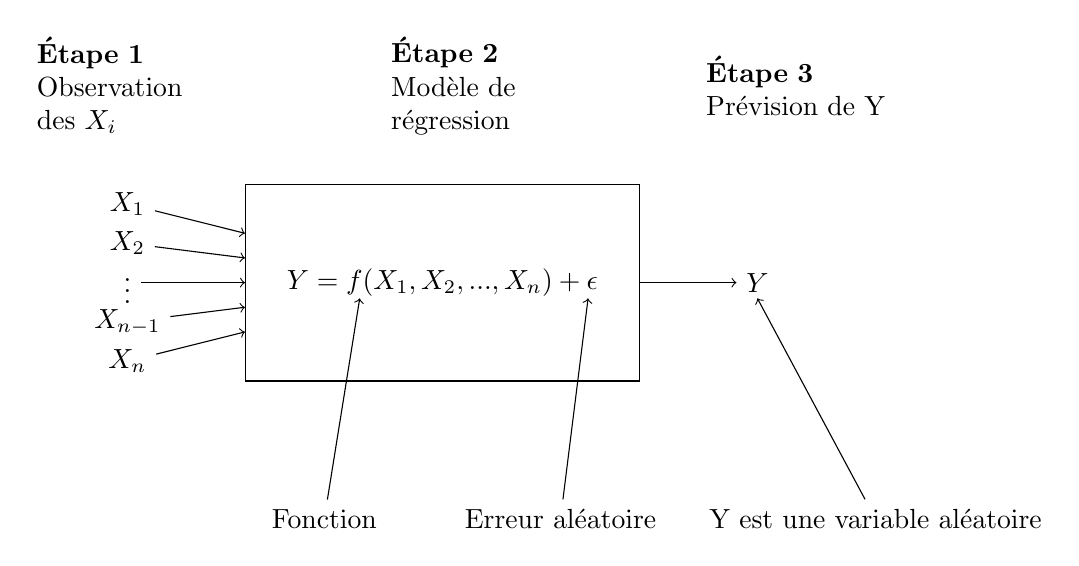
\begin{tikzpicture}
\node[block] (operator) at (4,1){$Y = f(X_1,X_2,...,X_n) + \epsilon$};
\node[text width = 2.3cm] at (0,3.5) {\textbf{Étape 1} \\
									Observation des $X_i$};
\node[text width = 2.3cm] at (4.5,3.5) {\textbf{Étape 2} \\
									Modèle de régression};
\node[text width = 2.3cm] at (8.5,3.5) {\textbf{Étape 3} \\
									Prévision de Y};										
\node (a) at (0, 2) {$X_1$};
\draw[->] ([right] a) --  (operator);
\node (b)at (0, 1.5) {$X_2$};
\draw[->] ([right] b) --  (operator);
\node (c)at (0, 1) {$\vdots$};
\draw[->] ([right] c) --  (operator);
\node (d)at (0, 0.5) {$X_{n-1}$};
\draw[->] ([right] d) --  (operator);
\node (e)at (0, 0) {$X_{n}$};
\draw[->] ([right] e) --  (operator);
\node (y)at (8, 1) {$Y$};
\draw[->] (operator) -- ([left] y);
\node (F)at (2.5, -2) {Fonction};
\draw[->] (F) --  (2.95, 0.8);
\node (E)at (5.5, -2) {Erreur aléatoire};
\draw[->] (E) --  (5.85, 0.8);
\node (Y)at (9.5, -2) {Y est une variable aléatoire};
\draw[->] (Y) --  (8, 0.8);
\end{tikzpicture}

Voici les deux types de régressions qui seront à l'étude durant la session:

\subsection*{Regression linéaire simple}
On cherche à prédire le salaire future des actuaires selon le modèle linéaire suivant,

\bigskip
%%% fig for the concept of regression operation
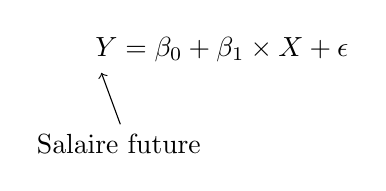
\begin{tikzpicture}[node distance=1.2cm]
\node (function) at (current page.center) {$Y  = \beta_0 + \beta_1 \times X + \epsilon$};
\coordinate[below of=function] (c);
\node[text width = 2.3cm, left of=c]  (Y) {Salaire future};
\draw[->] (Y) -- ([xshift=2mm, yshift=-3mm] function.west);
%\node[text width = 2.3cm] (X) at (8, -2) {Nombre d'années de scolarité};
%\draw[->] (X) --  (8,0);

\end{tikzpicture}

\end{document}
